\chapter{Receiver-Driven View-Dependent Streaming}
\label{c:rdstream}
\section{Introduction}
\label{s:dstream:intro}
    High resolution 3D models, such as artworks,
    cultural heritage, and scientific visualization are increasingly available over 
    the Internet. Stanford Digital Michelangelo Project \cite{levoy00digital},
    for example, provides high resolution 3D meshes of statues by Michelangelo.
    While current generations of commodity GPU already enables real-time rendering of these meshes, transmission of the meshes over the network remains
    a main bottleneck. For example, the Stanford model of the David statue, with 28 million vertices
    and 56 million triangles, needs more than 10 minutes to download at 1 Mbps
    even after compression. A natural choice to reduce the waiting time 
    is \emph{progressive streaming}, which allows
    users to see a coarse mesh quickly, with quality improved incrementally as
    more data arrives.

    \begin{figure}
    \centering
    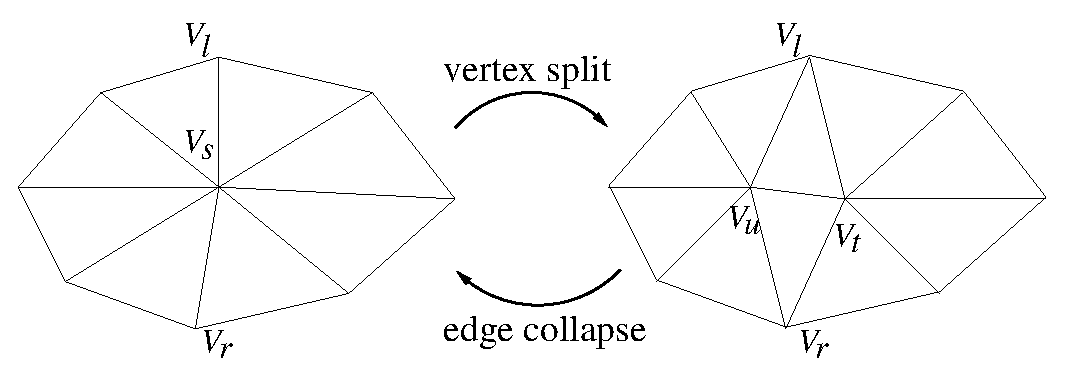
\epsfig{file = split.eps, height = 0.9in}
    \caption{Edge collapse and vertex split.
    This edge collapse removes one vertex by collapsing the edge $V_uV_t$ to a vertex $V_s$, and the
    vertex split reconstructs the edge from $V_s$. Vertices $V_l$ and $V_r$ are
    the cut neighbors of $V_s$.\label{dstream:split}}
    \end{figure}
    A commonly used representation of 3D models to support progressive streaming is
    progressive mesh \cite{237216}, which is based on two operations: 
    \emph{edge collapse} and \emph{vertex split}. 
    With the edge collapse operation,
    we can simplify a complex mesh into a simple base mesh
    by continuously collapsing one edge into
    a vertex. We reconstruct the original mesh
    by applying vertex split, the inverse of the edge collapse, in the
    reverse order of collapsing (see Figure \ref{dstream:split}). Therefore,
    progressive streaming can be implemented by sending the vertex
    splits as refinements after sending the base mesh.

    In progressive mesh streaming, it is desirable to increase the visual quality
    on the client side as quickly as possible.
    The ideal way is to send the vertex splits
    in the descending order of their contribution to
    mesh quality, commonly measured by the Hausdorff distance between
    the original and reconstructed mesh \cite{cignoni98metro}.
    As Hausdorff distance is view independent, 
    bandwidth may be wasted in sending invisible vertex splits
    before the visible ones. Moreover, even among the visible vertex splits,
    the view-independent metric cannot 
    reflect the real contribution to the visual quality of
    clients with different viewpoints. A vertex split that significantly
    changes a mesh may change the rendered image 
    only slightly.

    A better metric for visual contribution of a vertex split, which considers the receiver's viewpoint, is an image-based metric similar 
    to that proposed 
    by Lindstrom and Turk
    \cite{353995}, using the mean square error between the rendered images
    of the original mesh and reconstructed mesh.   
    %Lindstrom and Turk consider 
    %many viewpoints in their simplification since it is done off-line.
    %In the streaming case, we only need to consider the current viewer's
    %viewpoint. % since it is already known. Hence, 
    Based on this metric, \emph{view-dependent} streaming,
    in which vertex splits are sent in the descending order of 
    their contributions to the quality
    of rendered image, is introduced. 
    
    %can optimize the visual quality of the receiver side
    %during the transmission.
    %is a better choice.
    %because of two reasons. First, 
    %non-visible vertex splits will not be sent until all visible one are sent.
    %Second, the visible vertex splits can be sent in the descending order of 
    %their contributions to the quality of rendered image.

    \begin{figure}
    \centering
    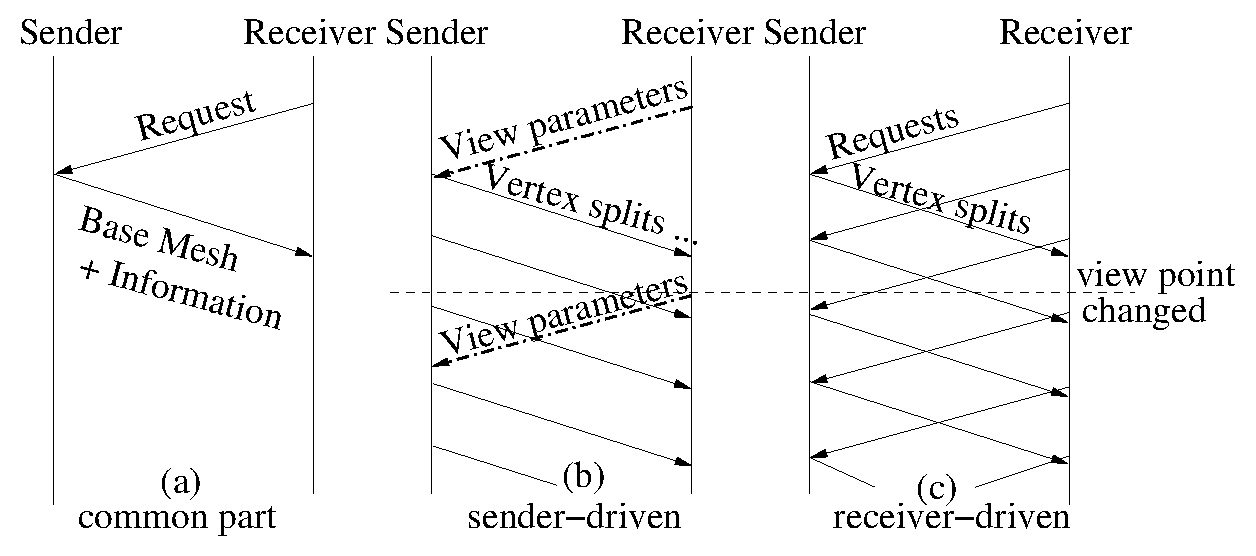
\epsfig{file = protocol.eps, height = 1.5in, width = 3.3in}
    \caption{Sender-driven protocol and receiver-driven protocol 
    \label{dstream:protocol}}
    \end{figure}
    In previous implementations of view dependent streaming
    \cite{To1999, 363375, progressive:Yang, kim:view, zheng:interactive}, 
    the server decides which vertex splits to send. In these implementations,  
    the client sends its
    viewing parameters to the server, and the server sends the chosen vertex splits after
    determining the visibility and the appropriate resolution of 
    different regions of the mesh (See Figure \ref{dstream:protocol}b).
    
    This sender-driven protocol, however, has two significant weaknesses.
    Firstly, it is not scalable to many receivers. Determining visibility of vertices
    and sorting the visible vertex splits based on their visual contributions
    are expensive operations. 
    %As a result, few of the existing schemes use sorting. In most implementations,
    %the visible vertex splits are sent in the reverse of collapse order, which is
    %often based on view-independent metrics. 
    Moreover, the sender needs to maintain
    the rendering state of each receiver to avoid sending duplicate data when receivers
    changes viewpoint.

    Secondly, due to the stateful design and huge computational requirements,
    the sender-driven approach cannot be extended easily to support 
    caching proxy and peer-to-peer architecture, two common solutions to scalability. It is not realistic
    to require each proxy or peer to provide much CPU time and memory. 
    Furthermore, a proxy or peer might not store the complete mesh.

    To address the above weaknesses, we propose a receiver-driven protocol,
    in which the receiver decides the sending order and explicitly requests
    the vertex splits. The sender simply sends the data requested 
    (See Figure\ref{dstream:protocol}c), so no expensive computation is needed.
    %In this protocol, the server is stateless and free of expensive computation.
    %We can exploit the client's GPU in determining the requesting order.
    Furthermore, the server is stateless, so
    existing cache proxy and peer-to-peer techniques can be applied.

    The receiver-driven protocol also reduces the size of data sent by the sender.
    In sender-driven protocols, for each vertex split, the sender has to send identifications
    to indicate which vertex to be split ($V_s$ in Figure \ref{dstream:split}),
    requiring at least $log_2{n}$ bits if $n$ vertices exist \cite{258843}. 
    In the receiver-driven protocol, however, the sender needs not send
    these identifications since the vertex splits can be sent according to
    the requesting order from the receiver. The identifications, sent
    by the receiver, consumes the down-link bandwidth 
    of the sender, which is often less likely to be the bottleneck than the up-link.

    Implementing the receiver-driven protocol is non-trivial. First, we need
    to assign each vertex a unique identification number so that the receiver
    can explicitly request vertex splits. Second, the receiver has to efficiently decide the
    importance of a vertex split based on partially received mesh.
    Although it is difficult for the receiver to accurately measure
    the visual importance of a vertex split, we find that estimation suffices
    in our scheme.  

    The main contributions of our work are as follows.  We
    propose a receiver-driven protocol of view-dependent streaming, which
    significantly reduces the CPU time of the sender
    and makes the sender stateless.  Our protocol exploits the receiver's 
    computing resources to approximate the optimal list of vertex splits to receive
    to improve the rendered mesh quality.  We also introduce an 
    algorithm to efficiently encode the receiver's requests.
    
    %Second, we reduce the transmission data
    %of the server by removing a significant part of data to its incoming channel. 
    %Third, we implement a prototype and evaluate its effectiveness with 
    %experiments.

    The rest of the paper is organized as follows.
    In Section \ref{s:dstream:related}, we introduce the related work. We briefly  
    review the traditional view-dependent approaches in Section \ref{s:dstream:terms}. 
    Then, we present the receiver-driven protocol 
    in Section \ref{s:dstream:protocol}.
    We evaluate our protocol in Section \ref{s:dstream:evaluation} 
    and conclude in Section \ref{s:dstream:conclude}.
\section{Related Work}
\label{s:dstream:related}
%\subsection{View-Dependent}
%\label{ss:view-dependent}
    The view-dependent approach first appeared as 
    a dynamic simplification method used for adaptive rendering of a complex 3D mesh
    \cite{258843, 258847}. Only vertex splits that contribute to the rendered
    image will be rendered, allowing real-time rendering of a complex mesh
    even with limited rendering capability.
    Besides progressive mesh, other multi-resolution representations, 
    such as vertex-clustering  and subdivision scheme,
    are used in view-dependent refinement systems \cite{245627, efficient:Alliez,602344}.

    Later, the view-dependent approach is used in progressive 
	streaming of 3D meshes.     In the scheme proposed by Southern et al. \cite{363375},  the client is stateless and
    maintains only the visible data. 
    To et al. \cite{To1999}
    and Kim et al. \cite{kim:view} proposed that received data are stored
    in the receiver even after they become invisible, 
    so they need not be resent when they are visible again. 
    In these papers, view-dependent approaches mainly aim at addressing
    limited rendering capability. 
    
    Yang et al. \cite{progressive:Yang} and
     Zheng et al. \cite{zheng:interactive}, on the other hand, use
     view-dependent streaming to address limited network bandwidth.
     Yang et al. proposed a scheme where the server chooses the appropriate resolution
     according to the available network bandwidth.
     Zheng et al. \cite{zheng:interactive} use prediction to
     reduce the effect of network latency and 
     compensate the round-trip delay with the rendering time.
     These systems use sender-driven approach and do not address
     server scalability issues.

    %\subsection{Reduce Dependency}
%\label{ss:reduce-dependency}
    The main challenge of these view-dependent schemes is 
    finding an appropriate subset of vertex splits to generate a 
    satisfactory rendered image on the client side.
    The flexibility of choosing a subset of vertices,
    hence, is crucial in view-dependent streaming. But this flexibility is
    restricted by the dependency among the vertex splits.
    For a manifold mesh, a vertex split operation depends on the existence of (a)
    the vertex to be split ($V_s$ in Figure \ref{dstream:split}), (b) two
    cut neighbors ($V_l, V_r$ in Figure \ref{dstream:split}). More dependencies exist if artificial
    folds are strictly forbidden \cite{258843, 258847}, but in this paper we
    ignore these dependencies since we can tolerate temporary folds in our scheme.

     To et al. \cite{To1999} further remove the second dependency.
     In their method, if a cut neighbor does not exist during a vertex split,
     its ancestor will be used as the cut neighbor instead.
     Kim and Lee \cite{kim01truly} improve this method so that the final mesh
     can keep the original connectivity. 
     %In their paper, when the original cut neighbor
     %is below the vertex front, its active ancestor is chosen instead. If the original
     %cut neighbor is above the vertex front, then we choose a proper active descendant of it.
     %As long as the two cut neighbors are not the same vertex, the vertex split can be processed.
     Kim et al. \cite{multiresolution:kim} propose a better scheme that enables
     an ordinary progressive mesh to be split in random order.
     This method is applied in our protocol to reduce the cut neighbor dependency
     and will be described in further details in Section \ref{s:dstream:protocol}.

     The flexibility in choosing split order, however, increases the difficulty
     in developing an effective encoding scheme. Most compression
     algorithms for progressive mesh %\cite{280834,319426, 614450, 383281,602153}
     choose a specific order of vertex splits
     to reduce redundancy by exploring the correlation
     between consecutive vertex splits.
     Moreover, compressed data can only be sequentially decoded
     so we cannot change the sending order. One solution
     proposed by Yang et al. \cite{progressive:Yang}
     is to divide the whole mesh into several segments and encode them
     separately to trade off between flexibility and compression efficiency.
     The weakness is that the size of the base mesh is relatively large
     since the original vertices in the border of segments are kept in the base
     mesh. Furthermore, the quality of the base mesh is uneven.

     Some related work \cite{multiresolution:kim, random:yoon}
     have proposed compression algorithms that allow random splitting of a mesh without
     sacrificing compression efficiency.   These algorithms are not designed for 
	 network transmission, but our scheme extended several ideas from Kim et al. \cite{multiresolution:kim}
     and applied them in view-dependent streaming.  

     The discussion above focuses on view dependent streaming of 3D meshes. View dependent streaming have also been used for other 3D data, such as terrain \cite{chang:terrains} and 3D scenes \cite{ott:tele}. 

\section{Current View-dependent\\ Approaches}
\label{s:dstream:terms}
    In this section, we briefly review the current view-dependent approaches since 
    they are the basis of our scheme.
   
    \begin{figure}
    \centering
    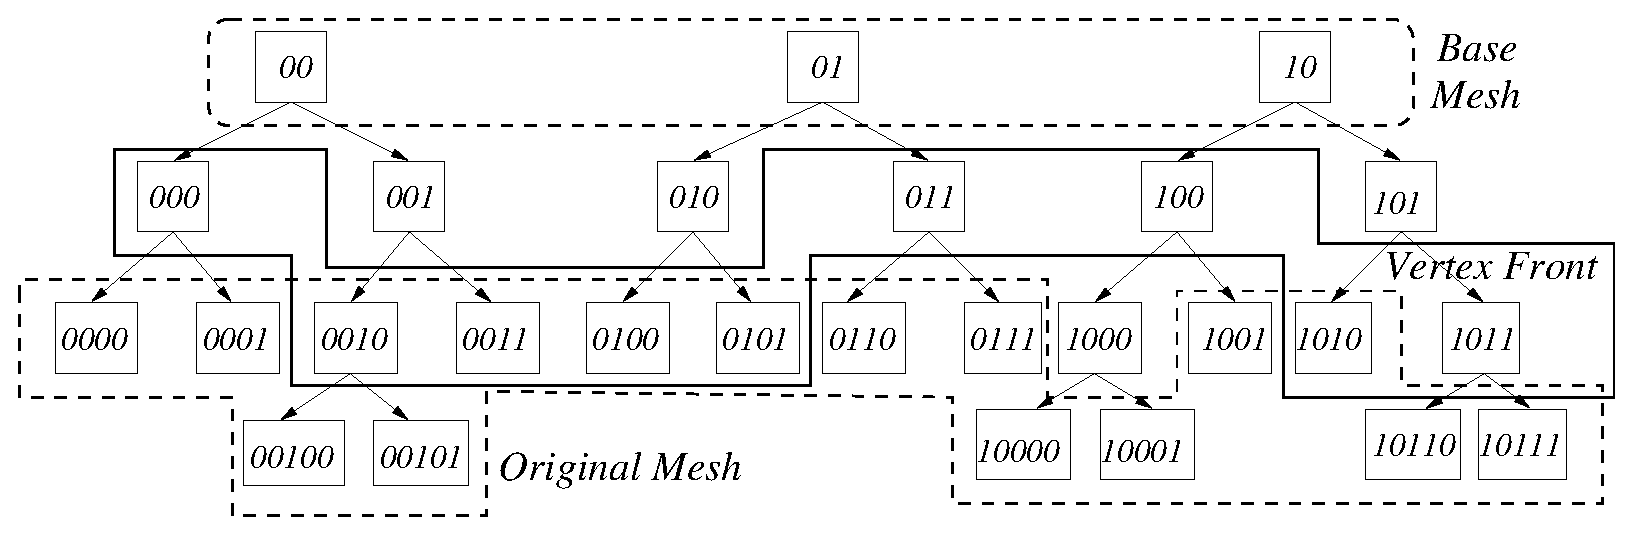
\epsfig{file = hierarchy.eps, height = 1.1in, width = 3.3in}
    \caption{Vertex hierarchy and vertex front. A rectangle represents a vertex and the number inside
    is its identification number, including tree ID and node ID.\label{dstream:hierarchy}}
    \end{figure}
    View-dependent systems often organize the vertices hierarchically.
    For example, Hoppe \cite{258843} represents
    parent-child relation among the vertices in a progressive mesh
    as a forest of binary trees, named \emph{vertex hierarchy},
    in which the root nodes are vertices in the base mesh, and
    the leaf nodes are vertices in the original mesh (see Figure \ref{dstream:hierarchy}).
    A vertex split replaces one vertex ($V_s$ in Figure \ref{dstream:split})
    by its two children ($V_u$ and $V_t$ in Figure \ref{dstream:split}).
    Thus, after applying some vertex splits,
    the result is a mesh lying between the original mesh and the base mesh.
    The set of vertices in current mesh is called \emph{vertex front}
    \cite{258843}
    (see Figure \ref{dstream:hierarchy}).% and vertices in the vertex front are \emph{active vertices}
    
    %When determining the visibility of vertex splits, a vertex split cannot be ignored when it
    %is not visible. If any of its descendants in the vertex hierarchy is visible,
    %the vertex split still needs to be applied. To avoid determining the visibility
    Due to dependencies among the vertices, visibility determination of a vertex cannot be based 
	on the vertex alone.
    An invisible vertex still needs to be split if any of its descendants is visible. 
    To avoid determining the visibility %\footnote{
    %For simplicity, in this paper determining the visibility also includes computing screen-space error.} for each
    recursively for all the descendants,
    %vertex in the vertex hierarchy is expensive. Therefore, 
    a common method is to use a bounding sphere to represent a vertex and all its descendants.
    Then, we can safely ignore a vertex split if its bounding sphere
    falls outside the view frustum.
    Similarly, a bounding cone of normal is used in back face culling \cite{258843}.
    %Therefore, some extra information to represent the bounding sphere
    %and bounding cone of normal is needed. Both Hoppe and Kim et al. \cite{258843, kim:view}
    %pre-compute the radius of the bounding sphere ($r_v$), the semi-angle of
    %the cone of normals ($\alpha$), and other two parameters
    %($\mu$ and $\delta$) for deciding the screen-space error
    %and store them with the vertex together.
    These bounding object-based methods are not appropriate
    in our receiver-driven protocol. First, it can only determine
    the visibility, but cannot sort the vertex splits by their visual contributions. 
    More importantly, the sender has to send
    these bounding parameters with the vertex splits, almost doubling 
    the data size.  We explain our solution to this issue in Section \ref{s:dstream:protocol}.
    %and the transmitted data size will be significantly increased. 
    %Since one vertex split has only five parameters, 
    %the identifications of two cut neighbors ($V_l$ and $V_r$) and the coordinations
    %of the new vertex ($x$, $y$, and $z$)
    %\footnote{We apply the half-edge collapse in our implementation
    %so that only coordinates of one vertex needs to be transmitted.},
    %adding four parameters almost doubles the data size. 
    %It is not acceptable since the network bandwidth
    %is considered as the main bottleneck.  

    After deciding the visibility, the sender sends the chosen vertex splits to the receiver.
    Six parameters are needed in a vertex split of a manifold mesh: the identification number
    (we call ID from now on) of the vertex to be split
    ($V_s$ in Figure \ref{dstream:split}) $Ids$, 
    the IDs for two cut neighbors 
    ($V_l$ and $V_r$ in Figure \ref{dstream:split}), $Id_l$ and $Id_r$,
    and the coordinates $x$, $y$, and $z$ of the right child ($V_t$ in
    Figure \ref{dstream:split}). Here, half collapse is used so $V_u$ remains at the same position
    of $V_s$. Many implementations use the sequence number of a vertex generated as its ID,
    but this method enforces the sender to be stateful since the sender has to remember 
    the sending order of each receiver.
    
    Kim and Lee \cite{kim01truly} proposed a new method, in which every vertex has
    an ID that is independent of the sending order. The ID of a vertex is a bit string
    with two parts: tree ID and node ID.
    Tree ID is the sequence number of the root of this tree in the base mesh, 
    and the node ID represents the path from the root to this vertex in the binary tree.
    For example, if the tree ID is `01', which is also the ID of
    the root vertex of this tree, the bit string `010' and `011' are the IDs
    of the left child and right child of the root vertex respectively. 
    A vertex hierarchy with the assigned IDs is shown in 
    Figure \ref{dstream:hierarchy}.
    
    Besides being independent of the sending order, another benefit of this scheme
    is that the IDs embed the hierarchy. Thus,  
    we can deduce the IDs of the ancestors and the descendants of each vertex. 
    For example, given `1001' as the ID of a vertex,
    we can deduce that `100' is the ID of its parent, `10010' is the ID of its left child and 
    `10011' is the ID of its right child. 
    This property frees the sender from sending the IDs of the two newly generated vertices
    ($V_u$ and $V_t$ in Figure \ref{dstream:split}), as they can be deduced by the receiver.
    
    The above property is also essential in splitting
    a progressive mesh in random order, in which the set of neighbors of a vertex
    during the decoding $\mathcal{N}'$ may not be $\mathcal{N}$, the set 
    during the encoding. If a cut neighbor with an ID of $Id$ %in $\mathcal{N}$
    is not in $\mathcal{N}'$, then either one of its 
    ancestors or at least one of its descendants must belong to $\mathcal{N}'$ \cite{multiresolution:kim}.
    In the former case, the ancestor is found and used as 
    the cut neighbor since its ID is the prefix of $Id$.  
    In the latter case, the descendants of the original 
    cut neighbor in $\mathcal{N}'$ are found since they all have $Id$ as their prefix.
    Kim et al. \cite{multiresolution:kim} propose a method to find out the 
    proper one as the cut neighbor and they show that despite using replacement
    in the vertex splitting, the original mesh can be 
    accurately reconstructed when all the vertex splits are applied.

    Kim et al. \cite{multiresolution:kim} also propose an algorithm
    to encode the IDs of two cut neighbors at about 12 bpv (bit per vertex) 
    and the coordinates $x$, $y$, and $z$ at about 21 bpv (with 12 bit quantization).
    Although their paper focuses on random access of local meshes, we find that this 
	method is useful in progressive streaming as well. 

\section{Receiver-Driven Protocol}
     \label{s:dstream:protocol}
	 We now present our proposed receiver-driven protocol
     for view-dependent progressive mesh streaming.
     We first introduce the process of transmitting 
     a progressive mesh. Then, we explain how the receiver decides the requesting order.
     Finally, we explain how we efficiently encode the request from the receiver.
     
     \subsection{Mesh Transmission} 
     A streaming session is initiated when the receiver requests for a specific
     mesh.
     The sender returns the complete base mesh and other necessary information
     (See Figure \ref{dstream:protocol}a) to the receiver.
     
     \begin{figure}
     \centering
     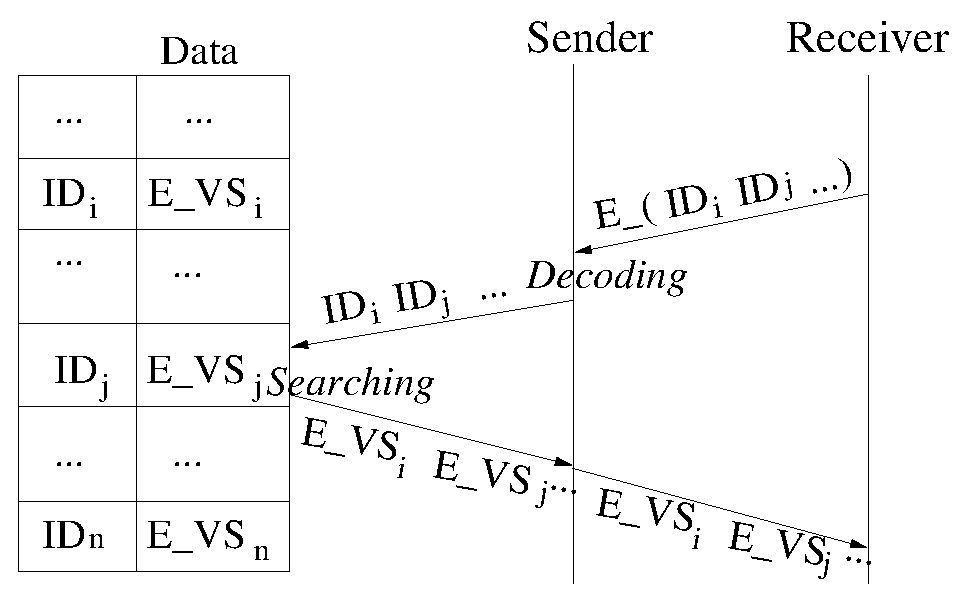
\epsfig{file =process.eps, height = 1.1in}
     \caption{The process of the sender in receiver-driven protocol. 
     E represents encoded data, and VS means vertex split. \label{dstream:process}}
     \end{figure}
     %After receiving the base mesh, 
     Then, the receiver determines
     the requesting order of the vertex splits based on the received base mesh, 
     encodes their IDs, and
     sends them to the sender. On the sender side, the vertex splits are stored
     in an associative array, which maps the ID to the vertex splits. 
     After receiving the encoded IDs from the receiver, 
     the sender decodes the IDs and searches for the vertex splits 
     in the associative array
     with IDs as the key values. The matched vertex splits
     are sent back to the receiver (See Figure \ref{dstream:process}). 
     The sender does only two things -- decode IDs and retrieve the 
     vertex splits, and is therefore stateless. 
     \subsection{Determining Visual Importance}
     \label{ss:dstream:visual}
     We now introduce how the receiver decides the requesting order. 
     We cannot directly use the mean square error between rendered images of 
     reconstructed mesh and original mesh to determine the order, 
     %image-based metric proposed by Lindstrom and 
     %Turk \cite{353995} 
     since we need to know the importance of a vertex 
     split before it is received. To overcome this problem, we estimate
     the importance of the vertex splits to request for based on the received
     mesh, using
     %We find that
     %estimation suffices %in the streaming case 
     %because some error in deciding the order will not affect the rendered
     %image.
     %
    \begin{figure}
    \centering
    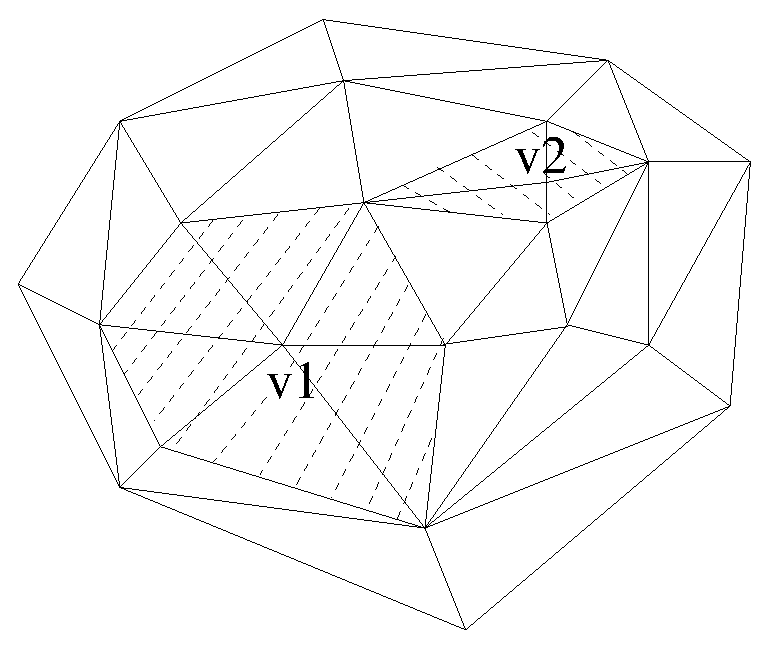
\epsfig{file =screen_area.eps, height = 1.0in}
    \caption{%Screen area of two vertices: v1 and v2.
    Rendered image on the receiver's screen. 
    The shaded are the screen area of vertex $V_1$ and vertex $V_2$.
    \label{dstream:screen_area}}
    \end{figure}
     %We use 
     the screen-space area of all the neighbor faces of a vertex as the 
     metric of its visual importance (see Figure \ref{dstream:screen_area}).
     The rationale is that if the screen area of a vertex ($V_1$ in Figure \ref{dstream:screen_area}) 
    is larger, it is likely the quality can
    be improved more by splitting this vertex. 
    Moreover, the screen-space area can be efficiently
    computed with the help of the GPU, by simply counting the
	number of pixels inside the faces in the frame buffer.
    %A simple method to compute the screen space of a triangle is 
    %to count how many pixels are inside it after rendering by analyzing
    %the frame buffer. 
    %We compute the screen-space area with the help of the GPU. 
    %First we assign each face in
    %the current mesh a unique color and render them. 
    %We can determine the visibility
    %and the screen-space area of each vertex by counting how many pixels with its color
    %are in the frame buffer, where the rendering result is stored. 
    %Then we add the pixel number to the face's three vertices. Thus, the
    %pixel number of a vertex (which is the sum of pixel numbers in its neighbor faces)
    %is proportional
    %to its screen-space area.
    %In brief, we estimate the visual importance of splitting a vertex by checking
    %at the projected area in the screen of the region occupied by this vertex and all its neighbors.
    
    Once the screen-space areas are computed, the receiver sends the requests 
	following the descending order of the 
    screen-space area. If the viewpoint changes, the visual importance will
    be re-computed and a new list of vertex splits will be requested. Since the received
    splits refine the mesh, the receiver recomputes the visual importance periodically
    to update the order even without viewpoint change. The refresh period, one second
    in our experiments, can be decided
    by the receiver based on mesh size and network bandwidth.

    The client can stop requesting once it finds that the rendering quality is sufficient.
    The receiver has the flexibility of continuing to request for the remaining vertex splits for future use.
    It can also pre-fetch some invisible vertices based on the prediction of future viewpoints.

    If the receiver stops requesting % for more vertex splits 
    when the visual quality is satisfactory, 
    it may miss some visible vertices since the visibility determination is just an estimate.
    Some invisible vertices may have potentially 
    visible descendants, but they will not be received if their parent has  
    no screen-space area. 
    Fortunately, in most cases, this kind of error is small and 
    tolerable (See the experiment results in Section \ref{s:dstream:evaluation}).
    If strict accuracy is needed, the receiver can choose to continue requesting 
    for the remaining vertex splits.  
		%Furthermore, some methods may reduce 
    %this kind of error, for example, by generating an appropriate base mesh or giving more
    %weight to the silhouette. We will consider these techniques in the future. 
    \subsection{Encoding of Vertex Splits and IDs}
    \label{ss:dstream:encoding}

    %Our progressive meshes are generated using OpenMesh\footnote{http://www.openmesh.org}. 
    %Here, we consider only manifold meshes and use half collapse in the simplification. We 
    %%The happy Buddha mesh is from Stanford University.
    %also use Kim's algorithm \cite{multiresolution:kim}
    %to code the IDs of two cut neighbors ($Id_l$ and $Id_r$).

	In this section, we explain how we encode the vertex splits 
	and the IDs of the requested vertex splits.  Note that, in 
	our work, we consider only manifold meshes and use half 
	collapse in the simplification.
    
	To encode a vertex split, we need to encode the IDs of the two
	cut neighbors and its $x$, $y$, and $z$ coordinates.
	We use Kim's algorithm \cite{multiresolution:kim} to code
	the IDs of the cut neighbors.
    To encode the coordinates, instead of encoding $x$, $y$, and $z$ directly, we encode $dx$, $dy$, and $dz$ with
    Huffman coding algorithm. Here $dx = x - x_0$, $dy = y - y_0$,
    and $dz = z - z_0$, and $x_0$, $y_0$, and $z_0$ are the coordinates of
    $V_s$, the vertex to be split. 
    The rationale to code the differences is that they have less entropy, especially
    for the later part of vertex splits, which only change the coordinates slightly.
    It is worth noting that all the encoding process are done off-line and the 
    encoded vertex splits are stored in the associative array, so the encoding will
    not increase overhead to the sender.

    According to the results of our experiments with the Stanford Happy Buddha model,
    we can quantize $dx$, $dy$, and $dz$ to 14 bits. 
    We need 11 bpv for both $Id_l$ and $Id_r$ 
    and 20 bpv for all three of $dx$, $dy$, and $dz$ on average.
    It is worth noting that more bits are needed for $dx$, $dy$, and $dz$ 
    for the earlier vertex splits (about 30 to 35 bpv)
    since their values are larger. 
    The number of bits needed decreases significantly for later part of the vertex splits
    as $dx$, $dy$, and $dz$ decrease. We think that compressing $x$, $y$, and $z$ 
    based on better prediction techniques may further increase the 
    efficiency and it will be an interesting topic of future work.

    We now introduce how we encode the vertex split IDs, 
    which need 32 bpv without compression.  
    %First we choose the number of vertex identifications to be packetized appropriately
    %such that their vertex splits after encoded will no exceed
    %the size of an Ethernet packet (often 1500 bytes). The reason is to
    %reduce the dependency among packets so that
    %one packet loss will not affect the decoding of another packet.
    %A previous paper \cite{1291399} has discussed the importance to reduce the dependency
    %among the packets.
    The two parts of an ID, tree ID and node ID, are encoded separately.  We use a bit string \textit{code} to store the encoded result.
    First, we sort the IDs in a packet according to the tree IDs, in increasing order. 
    Then, we store the first tree ID to \textit{code} and 
    store each of the following tree ID as the difference from the previous tree ID.
    Since they are sorted, the differences are positive and relatively small numbers.

    \begin{figure}
    \centering
    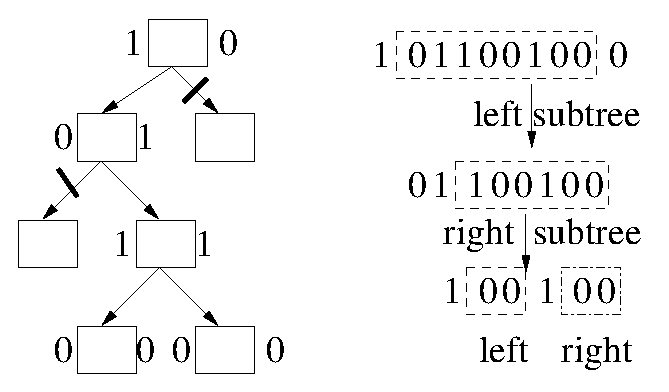
\epsfig{file =encode_id.eps, height = 1.0in}
    \caption{The code of ID of the bottom two
    vertices is 1011001000. 
    \label{f:dstream:encode_id}}
    \end{figure}
    \begin{algorithm}
    \caption{Encoding Vertices in One Tree.
    Input: IDs of vertices in a tree to be split;
    Output: a bit string as the \emph{code}.\label{a:dstream:encode_id}}
    \begin{algorithmic}
    \IF{no vertex needs to be encode in the left subtree}
        \STATE append `0' to \emph{code};
    \ELSE
        \STATE append `1' to \emph{code};
        \STATE encode the left subtree;
    \ENDIF
    \IF{no vertex needs to be encode in the right subtree}
        \STATE append `0' to \emph{code};
    \ELSE
        \STATE append `1' to \emph{code};
        \STATE encode the right subtree;
    \ENDIF
    \end{algorithmic}
    \end{algorithm}
    Next, we encode the node IDs in a tree into a bit string with 
    a recursive algorithm (See Algorithm \ref{a:dstream:encode_id}).
    In brief, we use two bits to represent whether one or more descendants need
    to be split (`1' for yes and `0' for no)
    in the left subtree and right subtree respectively. 
    In the example shown in Figure \ref{f:dstream:encode_id}, for the root vertex, since at least one vertex
    in the left subtree needs to be split, we append `1' to the code and encode the
    left subtree. At the root of the left subtree, since no vertex needs to split in its left
    subtree, we append `0' and check its right subtree. Vertices to be split exist in the right
    subtree, so we append `1' and encode its right subtree recursively as `100100'. 
    Finally, we return back to the root and append `0' since 
    no nodes in the right subtree needs to be split. 
    Therefore, the result is `1011001000'.
        
    During decoding, the sender traverses the tree according to the bits of the code. 
    The bit `1' means to decode the subtree and the bit `0' means to stop and return.
    If a vertex has no descendants that needs to be decoded, then this vertex is split. 
    Decoding is done when the procedure returns to the roots.
    
    The advantage of this method is that the code length is variable and the 
    length can be determined without extra flags. The coding efficiency depends
    on how many vertices need to be split inside a tree. Two bits
    are assigned to each vertex traversed during the encoding
    (including the vertices to be split and their ancestors in their path
    to the roots). Thus, the code efficiency is higher when more vertices in one tree
    are encoded since the overhead is amortized across the vertices. 
    %In worst case, we traverse $d$ nodes just for encoding $1$ vertex,
    %so in maximum $2d$ bits are needed for a node ID. Here, $d$ is
    %the depth of a node. In best case, all leaves are needed to be split. 
    %Assuming there are $m$ leaves, then the
    %total traversed nodes are $2m-1$ and the total bits are $4m-2$.
    %Therefore, in minimum about $4$ bits is needed
    %to encode a node ID. 
    %
    %Due to the limited space, we omit the decoding algorithm
    %here. It can be deduced from the encoding algorithm.

    We can further reduce the data size for some receivers whose up-link (receiver to
    sender link) bandwidth is much less than the down-link (sender to receiver link) 
    bandwidth. These receivers can request the sender to send not only the vertex split
    for the requested vertex but also the vertex splits for its descendant.
    For example, if the receiver sends an ID 
    `10010', the sender can send vertex splits for `10010', `100100', `100101'.
    The receiver can explicitly indicate in the packet how many descendants to send. This method 
	also allows the server to better utilize its outgoing bandwidth by filling the pipeline when RTT between the server and the client is high.

\section{Evaluation}
In this section, we introduce the experiments results to evaluate our protocol.
We choose two computers on a LAN as the sender and the receiver. 
We use several meshes from Stanford University in our experiments, but we only
present the result of Happy Buddha in this paper due to the space limit.
\label{s:dstream:evaluation}
\subsection{CPU Usage of the Sender}
\begin{table}[b]
\centering
\begin{tabular}{|c|c|c|}
\hline
&Sender-driven &Receiver-driven\\
\hline
send    base mesh           & 1.40s & 1.13s  \\
%receive encoded IDs         & -     & 0.06s  \\
decode  IDs                 & -     & 1.55s  \\
search vertex split         & 1.85s  & 1.85s \\
%receive the view parameters &       & -      \\
%traverse vertex hierarchy   &   & - \\
determine visibility        & 0.41s & - \\
update vertex front         & 1.41s & - \\
encode IDs                  & 0.94s & - \\
%send data                   &       & 0.10s  \\
others                      &0.16s  & 0.16s\\
\hline
\end{tabular}
\caption{Comparison of CPU usage of the sender.
\label{t:dstream:cpu}}
\end{table}
We compare the CPU usage of the sender in sender-driven
protocol and receiver-driven protocol after all vertex splits
are received (see Table \ref{t:dstream:cpu}). 
The implementation of the sender-driven protocol is modified from
our receiver-driven protocol using the visibility determination
algorithm from Kim et al. \cite{kim:view}. % by adding encoding scheme.
In both experiments, the client changes its viewpoints exactly the
same way.
A computer with an Intel Core 2 Duo 2.4 GHz CPU and 4 GB memory is
used as the sender.  We profile the code five times 
with Google CPU profiler and take the average value.
%We transmit
%the Stanford Happy Buddha mesh with both protocols and compare
%the CPU time used by the servers. 
We can see that the receiver-driven protocol reduces the CPU usage
of the sender by 24\% since we remove the processes for determining the visibility and updating the vertex front on the sender. 
\subsection{Transmitted Data Size}
During transmissions of the Happy Buddha model (542652 vertex splits) using 
the receiver-driven protocol, 1.83 MBytes are sent from the receiver
to the sender as vertex split IDs, and 2.21 MBytes are sent from the sender 
to the receiver as vertex splits. 
Thus, on average, IDs cost 27 bpv and vertex splits cost 32 bpv.
If sender-driven protocol is used, both IDs and 
vertex splits are sent from the sender to the receiver, so the total data 
sent by the sender are 4.04 MBytes. Thus, by moving IDs from the down-link to up-link, we reduce the outgoing bandwidth consumption of the sender by more than 40\%.

Reducing the outgoing data size also shortens the downloading time.
In the receiver-driven protocol, although the total transmitted size remains
the same, about 40\% of the data are now transmitted in the up-link of
the client.  On duplex links where up-link transmission can occur concurrently with down-link
transmission, the total transmission time reduces by about 40\% as well.
%\footnote{Recall that users with low up-link bandwidth can request a packet with its descendants at once to reduce the up-link data rate.}. 
%Assuming that the server keep sending data at $R$ Bps, IDs cost $S_i$ bytes,
%and Vertex splits cost $S_v$ bytes. Then sender-based protocol needs
%$t_s = \dfrac{S_i + S_v}{R}$ to download the mesh, but the receiver-driven protocol
%needs only $t_d = \dfrac{S_v}{R} + t$, where $t$ is the time to send the first several
%packets of IDs before the first packet of vertex splits arrive,
%since the sending of remaining IDs are parallel with the downloading. 
%Because $t$ is much less than $\dfrac{S_v}{R}$, $t_d$ is much shorter than
%$t_s$. 
\subsection{Quality}
%   \begin{figure}
%    \centering
%    \epsfig{file =psnr.eps, height = 2.6in, angle = 270}
%    \caption{
%    Relation between PSNR value and received vertices\label{f:psnr_vertices}}
%    \end{figure}
%In progressive streaming, the optimal sending order generates
%the fastest growing of rendered image quality. Therefore,
%we check the effectiveness of our protocol by checking the
%quality increasing curves. We choose the PSNR value as the 
%metric of rendered image quality. In Figure \ref{f:psnr_vertices}, 
%we can see the relation between PSNR value and the received vertices
%number. The view-independent streaming sends a lot of invisible vertex splits, 
%so the quality increases much slower than the view-dependent streaming.

   \begin{figure}
    \centering
    \epsfig{file =vps2.eps, height = 2.6in}
    \caption{
    The upper row shows the rendered images, and the lower row shows 
    the reconstructed meshes when the quality of rendered images is acceptable.
    %For each mesh, left: front side, right: back side.
    The rectangles over the images represent the viewable areas of the user.
    \label{f:dstream:vps}}
    \end{figure}
   \begin{figure*}
    \centering
    \begin{tabular}{ccc}
    \epsfig{file =psnr2.eps, height = 2.2in, width = 1.5in, angle = 270}
    &
    \epsfig{file = psnr22.eps, height = 2.2in, width = 1.5in, angle = 270}
    &
    \epsfig{file = psnr23.eps, height = 2.2in, width = 1.5in, angle = 270}
    \\
    \\
    View Point 1
    &
    View Point 2
    &
    View Point 3
    \\
    \end{tabular}
    \caption{
    How PSNR changes with amount of received data.  We cut off the curve when PSNR = 35 as its value approaches infinity when enough data are received.
    \label{f:dstream:psnr_bytes}}
    \end{figure*}
We follow Lindstrom and Turk \cite{353995} and use an image-based metric
to evaluate the quality of a reconstructed mesh. It is reasonable since
the representation of a 3D mesh on the receiver side is the 2D rendered image.
In this paper, we use the PSNR value of the rendered image as the metric,
with the rendered image of the original mesh as the reference. 

Figure \ref{f:dstream:psnr_bytes} shows how PSNR changes with the amount of data received. 
Assuming constant transmission rate, this figure
also shows how PSNR value changes with time. 
We do the experiments with three different viewpoints (see Figure \ref{f:dstream:vps}). 
In receiver-driven protocol, the quality grows much faster than sender-driven protocol because 
data transmitted are reduced.
View-independent streaming, although having the highest 
compression ratio (20 bpv \cite{383281}), 
wastes majority of bandwidth in sending invisible
vertex splits, so it increases the quality at a slower rate, 
especially when only a small part of the mesh is visible (e.g. View Point 3). 

\if 0
\begin{table}
\centering
\begin{tabular}{|c|c|c|c|}
\hline
       & receiver-driven & sender-driven & view-independent\\
\hline
viewpoint1 &    718K     &   1383K      &     1332K       \\
\hline
viewpoint2 &    267K     &    511K      &     1302K       \\
\hline
viewpoint3 &    113K     &    200K      &     1280K       \\
\hline
\end{tabular}
\caption{The bytes needed to achieve PSNR > 30.\label{t:dstream:psnr30}}
\end{table}
Now we assume PSNR value being 30 as the acceptable quality. Table \ref{t:dstream:psnr30} shows
the bytes needed to be received to achieve the acceptable quality, and Figure \ref{f:dstream:vps}
shows the rendered images and reconstructed meshes.
Table \ref{t:dstream:psnr30} shows that our protocol can achieve the acceptable quality much quicker. 
\fi
\begin{table}
\centering
\begin{tabular}{|c|c|c|c|}
\hline
             & View Point 1 & View Point 2 & View Point 3 \\
\hline
error pixels &   305           &      226       &     115         \\
\hline
proportion   & 0.12\%             &   0.09\%           &  0.05\%           \\
\hline
PSNR         &   37.8        &    38.3        &    40.6        \\
\hline
\end{tabular}
\caption{Errors of rendered mesh when only visible vertices are split.
There are 250,000 (500$\times$500) pixels in total.\label{t:dstream:error}}
\end{table}
As we explained in Section \ref{s:dstream:protocol}, if the receiver stop requesting vertex splits after all the visible splits received,
some potentially visible vertices may not be generated.
We use two methods to compare the rendered images between the original mesh and the reconstructed mesh when all visible vertices
are split. One is to find
how many pixels are different and the other is to compute the PSNR value. 
Table \ref{t:dstream:error} shows that the error is negligible.
% -- less than 0.12\% of the pixels are different and the PSNR values of the rendered images are at least 37.8.
%add figures and explanation here.
\section{Conclusion}
\label{s:dstream:conclude}
\if 0
In traditional view-dependent systems,
senders decide which refinements to send, so they are
stateful and need expensive computation. %Not only the CPU time but also
Besides the CPU time,
the output bandwidth also make the sender not scalable to many receivers,
since cache proxy and peer-to-peer system cannot be applied easily.

We propose a receiver-driven protocol to address the above weakness.
The main finding of us is that %the accuracy of rendered image is not
%strictly required during previewing,
receivers can estimate the visual importance of a vertex split, even before
it is received, based on the current received mesh. Moreover, we can exploit the GPU
in determining the visibility and visual importance of vertices.

In our protocol, the sender is stateless,  so the receiver can easily
switch from different senders during transmission or even simultaneously
download from multiple senders. Therefore, we can easily apply
the cache proxy or peer-to-peer techniques to solve the scalability problem. 

Another benefit is that the receiver explicitly requesting the vertex splits
frees sender from sending the IDs of vertex splits. As a result, the
transmission data on the down-link of the sender is significantly reduced. 
\fi
In this paper, we propose the receiver-driven approach for view-dependent 
streaming of 3D meshes.  Our preliminary study shows that the approach
is promising in reducing the sender's resource requirements, both in CPU and
outgoing bandwidth.  The stateless nature of the sender in our approach makes
it a natural choice in peer-to-peer mesh streaming and caching proxy.
We plan to study how our protocol can be applied in these two areas.  Our
protocol can also be easily extended to support streaming of a scene with
multiple mesh objects.
%This paper is the first step in receiver-driven approach
%and many improvements can be done in future. 
%For example, better visual importance estimating algorithms may be
%developed later. Progressively improving the geometrical precision
%may be used to reduce the bandwidth requirement in the initial
%stage. Peer-to-peer system of progressive mesh streaming can be
%designed based on our idea. Moreover, our scheme can be further
%extended to progressive streaming of a complex scene instead of just one
%object. 
\section*{Acknowledgment}
This work is supported by National University of Singapore Academic Research Fund R-252-000-306-112.
